\chapter{Descrição geral do projeto}
\section{Cadeia de Abastecimento de Cerveja}


O projeto consiste na simulação e análise de uma cadeia de abastecimento de cerveja e foi didivido em duas fases. A primeira fase consistiu em formar vários grupos de alunos, em que cada um dos grupos representava uma cadeia de abastecimento e o cliente seria representado pela docente. Formando uma cadeia de abastecimento com a seguinte estrutura: 

\begin{figure}[tbph]
	\centering
	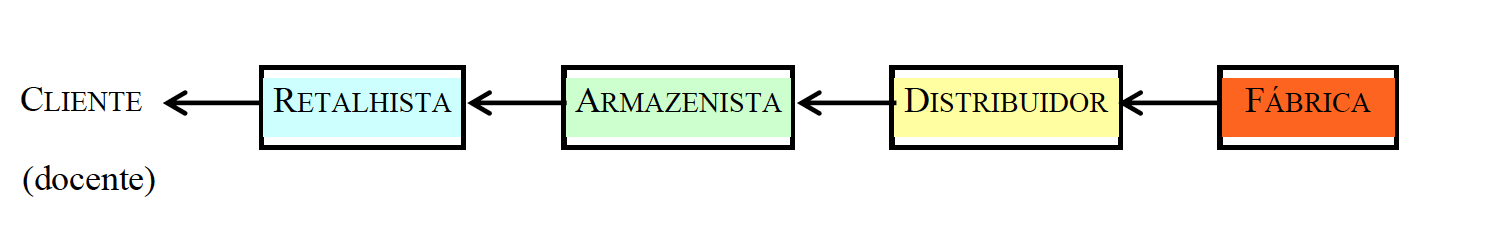
\includegraphics[scale=0.5]{imagem/estrutura.png}
	\caption{Estrutura da cadeia de abastecimento}
	\label{fig:cominicacaoservidorcliente}
\end{figure}

Ao longo da simulação, cada equipa teria apenas conhecimento das encomendas que de semana a semana a equipa localizada a jusante vai pedindo. Com base nesta informação cada equipa deverá encontrar um algoritmo de gestão de stock, de modo a satisfazer os pedidos do cliente, e obter o melhor desempenho possível em termos de custo total de operação no final de todo o processo. O prazo establecido para a entrega de todas as encomendas é de 2 semanas. 

Para o cálculo de atualização do registo interno do inventário usaram-se as seguintes fórmulas: 

$emTransito1(t) = emTransito2(t-1)$

$stockAbertura (t) = stockFecho(t-1) + emTransito1(t-1)$

$despacho = min [(pedido + porDespachar); stockAbertura]$

$porDespachar(t) = porDespachar(t -1) + [pedido(t) - despacho(t)]$

$stockFecho = stockAbertura - despacho $
\vspace{1cm}

Os custos associados serão: 
\begin{itemize}
	\item Custo de posse = 1\euro/artigo/semana
	\item Custo de quebra = 2\euro/artigo/semana 
	\item Custo de encomenda = 5\euro/encomenda 
	\item Custo de produção = 5\euro   (apenas na Fábrica)
\end{itemize}



